\chapter{调制识别的理论基础}\label{chap:intro}
\markboth{第二章\ \ 调制识别的理论基础}{}
% ### 章节大纲

% 1. **引言**
%    - 研究背景与目的
%    - 章节内容概述

% 2. **数字调制信号模型**
%    - 数字调制的基本原理
%    - 常见数字调制类型及其数学模型
%    - 调制信号的图形表示

% 3. **传统调制识别方法分析**
%    - 传统方法概述
%    - 各种传统方法的优势与局限性
%    - 传统方法的历史贡献

% 4. **深度学习在调制识别中的应用**
%    - 深度学习方法概述
%    - 特征提取能力与应用优势
%    - 深度学习方法的实际应用案例

% 5. **宽带信号处理的挑战与解决方案**
%    - 宽带信号处理的问题阐述
%    - 多陪集采样原理及应用
%    - 压缩感知理论在调制识别中的应用

% 6. **数据集介绍与评估方法**
%    - 常用数据集的介绍
%    - 数据集在调制识别评估中的作用
%    - 实验设计与性能评估标准

% 7. **总结**
%    - 本章重点回顾
%    - 对后续研究章节的铺垫

% 通过本章的详细介绍,读者将能够全面理解调制识别领域的理论基础,为深入了解后续的具体研究方法和实验设置打下坚实的基础。



\section{引言}\label{sec:background}
% 本章旨在为调制识别领域的理论基础提供全面的介绍。首先,我们将对数字调制信号模型进行详细阐述,通过数学公式和图像两个角度对常见的数字调制模式进行全面描述,为后续调制识别任务建立主观认知基础。传统调制识别方法是研究的重要组成部分,本章将从多个角度对传统方法进行分析,深入挖掘其优缺点,为后续工作提供深刻启发,突显传统方法在调制识别领域的历史贡献。通过对传统方法的全面了解,我们能更好地把握调制识别问题的本质,为提出更创新、更高效的解决方案奠定坚实基础。

% 随后,我们将重点介绍目前主流的深度学习方法在调制识别中的应用。深度学习在自动调制识别领域取得显著进展,其强大的特征提取能力为调制识别任务带来新的视角。通过深入学习深度学习理论,我们能更好地理解并应用这一跨学科领域的理论,为实际问题的解决提供新的思路。本课题的创新点之一是宽带调制信号的识别与解调,为了解决采样与存储的难题,我们引入了压缩感知理论,这部分将详细阐述多陪集采样的基本原理及其在宽带调制信号处理中的应用,为后续章节的具体方法和算法提供理论支持。最后,我们将介绍一些常用的数据集,这些数据集将为后续内容提供坚实的实验基础。通过对这些数据集的了解,我们能更全面地评估不同方法在真实场景中的性能,并为调制识别领域的实证研究提供可靠的数据支持。在理论基础的系统构建后,我们将深入探讨调制识别方法的设计与实现,为该领域的进一步研究奠定扎实基础。

本章旨在全面介绍调制识别领域的理论基础,既包括数字调制信号模型的深入阐述,也包括对传统调制识别方法和当前的深度学习方法的详尽分析。通过这一综合性的理论框架,本研究为后续工作建立了坚实的基础,特别是针对宽带调制信号的识别与解调所面临的挑战。

首先,本章将详细描述数字调制信号模型,通过精确的数学公式和直观的图像展示来全面描述常见的数字调制模式。这一部分的目的是为读者建立关于不同调制类型的清晰认识,为理解调制信号的复杂性和多样性提供必要的背景。
% 接着,本章将深入探讨传统调制识别方法。这些方法的历史和发展对于理解调制识别问题至关重要。我们将从多个角度分析这些方法,深入挖掘它们的优势和局限,从而为后续工作提供深刻的见解。此外,通过突出传统方法在调制识别领域的历史贡献,本章将展示这些技术是如何为现代方法铺平道路的。
在第一章中已经详细地介绍了传统调制识别方法的基础以及相应的弊端,本章将转向目前主流的深度学习方法在调制识别中的应用。深度学习的引入在自动调制识别领域引发了一场变革,特别是其在特征提取方面的强大能力。我们将探讨深度学习如何为解决复杂的调制识别问题提供新的思路和方法。为了解决宽带调制信号处理中的采样和存储挑战,本章将详细阐述多陪集采样的基本原理及其在宽带信号处理中的应用。通过引入压缩感知理论,本研究为高效处理宽带信号提供了理论支持。这一创新点是本研究的重要组成部分,将在后续章节中进一步发展。最后,本章将介绍一些常用的数据集,并解释这些数据集在评估不同调制识别方法中的作用。这些数据集不仅为实证研究提供了坚实的基础,也使我们能够全面评估各种方法在实际应用中的性能。

通过这些内容的系统介绍,本章为探讨调制识别方法的设计与实现奠定了坚实的理论基础,并为该领域的进一步研究提供了必要的背景和知识。

\begin{figure}
    \centering
    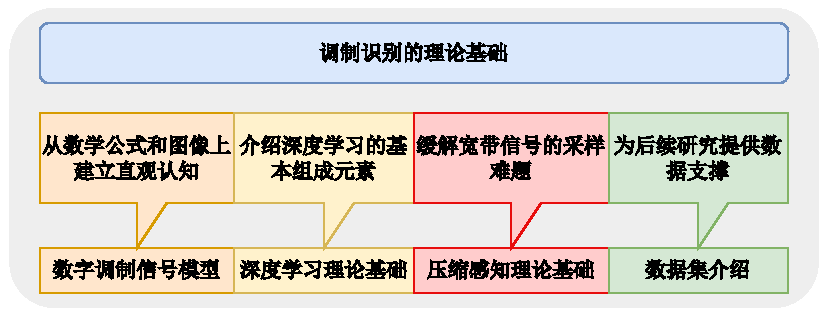
\includegraphics[width=\textwidth]{Image/chap2_map.pdf}
    \caption{本章大纲}
    \label{fig:outline2}
\end{figure}

\section{数字调制信号模型}\label{sec:background}
数字通信是现代通信技术中的一种核心模式,其主要原理在于将离散的数字信号源转换为用于传输的时间连续信号。相较于传统的模拟通信,数字通信系统展现出显著的优势,例如更高的信号传输质量和更强的干扰抵抗能力。特别是在可靠性方面,数字信号可以通过编码来增强,使其在复杂的通信环境下保持较高的传输稳定性。此外,数字信号的离散性质使得它们易于通过计算机进行处理,从而大幅提升了通信系统的效率和灵活性。

在数字通信系统中,调制技术起着至关重要的作用。它涉及到将数字数据转换为适合在物理媒介(如无线电波)上传输的信号的过程。主要的数字调制技术包括幅移键控(Amplitude Shift Keying, ASK)、频移键控(Frequency Shift Keying, FSK)、相移键控(Phase Shift Keying, PSK)和正交振幅调制(Quadrature Amplitude Modulation, QAM)。这些调制技术通过改变载波信号的不同特性(如幅度、频率或相位)来代表数字数据。

本节将深入探讨这些数字调制技术的原理和特点,为理解它们在调制识别中的应用提供坚实的理论基础。通过对这些调制技术的详细介绍,本文旨在建立对数字调制过程的全面理解,为后续探讨调制识别的先进技术和方法奠定基础。

\subsection{幅移键控}\label{sec:background}
% 在幅移键控中,数字信息被转换为不同的振幅水平。信号的振幅随着数字信号的变化而改变,从而产生调制后的信号,其数学表达式为:
% \begin{equation}
%     s_{MASK}(t) = A \sum_n a_n g_T (t-nT_s) \cos(2\pi f_c t),
% \end{equation}
% 公式中,$a_{n} \in \{\pm 1, \pm 3, \dots, \pm(M-1)\}$。

% 通常,ASK用于调制二进制信号,其中0和1分别对应于两个不同的振幅水平。 如果要发送数字1,则信号振幅增加到特定水平;如果要发送数字0,则信号振幅减小到另一个特定水平。接收端测量接收到的信号的振幅,并根据振幅的不同来判断发送的是0还是1。
% 图~\ref{fig:ASK}展示了ASK的示意图。

幅移键控(ASK)是一种基本的数字调制技术,它通过改变信号的振幅来传输数字信息。在ASK中,数字信号被转换成不同的振幅水平,从而实现数据的传输。这种调制技术的关键在于,它直接调节载波信号的幅度,以代表数字数据。ASK信号的数学表达式如下:

% ### 数学表达式
\begin{equation}
    s_{MASK}(t) = A \sum_n a_n g_T (t-nT_s) \cos(2\pi f_c t),
\end{equation}
其中,\( A \) 是载波的振幅,\( a_n \) 是表示数字信息的振幅系数,\( g_T(t) \) 是脉冲形状函数,\( T_s \) 是符号周期,\( f_c \) 是载波频率。\( a_n \) 的取值通常是 \(\{\pm 1, \pm 3, \dots, \pm(M-1)\}\),这里的 \( M \) 表示振幅的不同水平数量。

% ### 二进制ASK
在二进制ASK中,只使用两个振幅水平来表示数字0和1。例如,当需要传输数字1时,信号的振幅被设置为较高的水平;相反,传输数字0时,则将振幅设置为较低的水平。接收端通过测量接收信号的振幅并比较预定义的阈值,来确定传输的是0还是1。其主要有如下特点:

% ### ASK的特性与适用场景
简单性:ASK调制技术因其实现简单而被广泛应用,尤其适用于带宽受限和系统复杂度要求低的通信系统。

功耗:由于ASK直接调制振幅,因此在某些情况下可能比其他调制技术(如FSK或PSK)更耗电。

抗干扰能力:ASK对噪声较为敏感,特别是在信号强度低的情况下,噪声可能会导致错误的数据解读。

适用范围:ASK常用于短距离和低速率的通信,例如无线射频识别(RFID)和一些无线传感器网络。

% ### 总结
幅移键控作为一种基础的数字调制技术,在特定的应用场景下具有其独特的优势。尽管存在一些局限性,如对噪声的敏感性和较高的功耗,ASK仍然是数字通信中不可或缺的一部分。对ASK技术的深入理解,对于全面掌握数字调制的理论和实践具有重要意义。图~\ref{fig:ASK}所示为幅移键控的示意图,展示了4ASK中不同数字状态对应的振幅变化。通过这种直观的表示,可以清晰地理解ASK调制信号的基本原理和特点。

\begin{figure}[htbp]
    \centering
    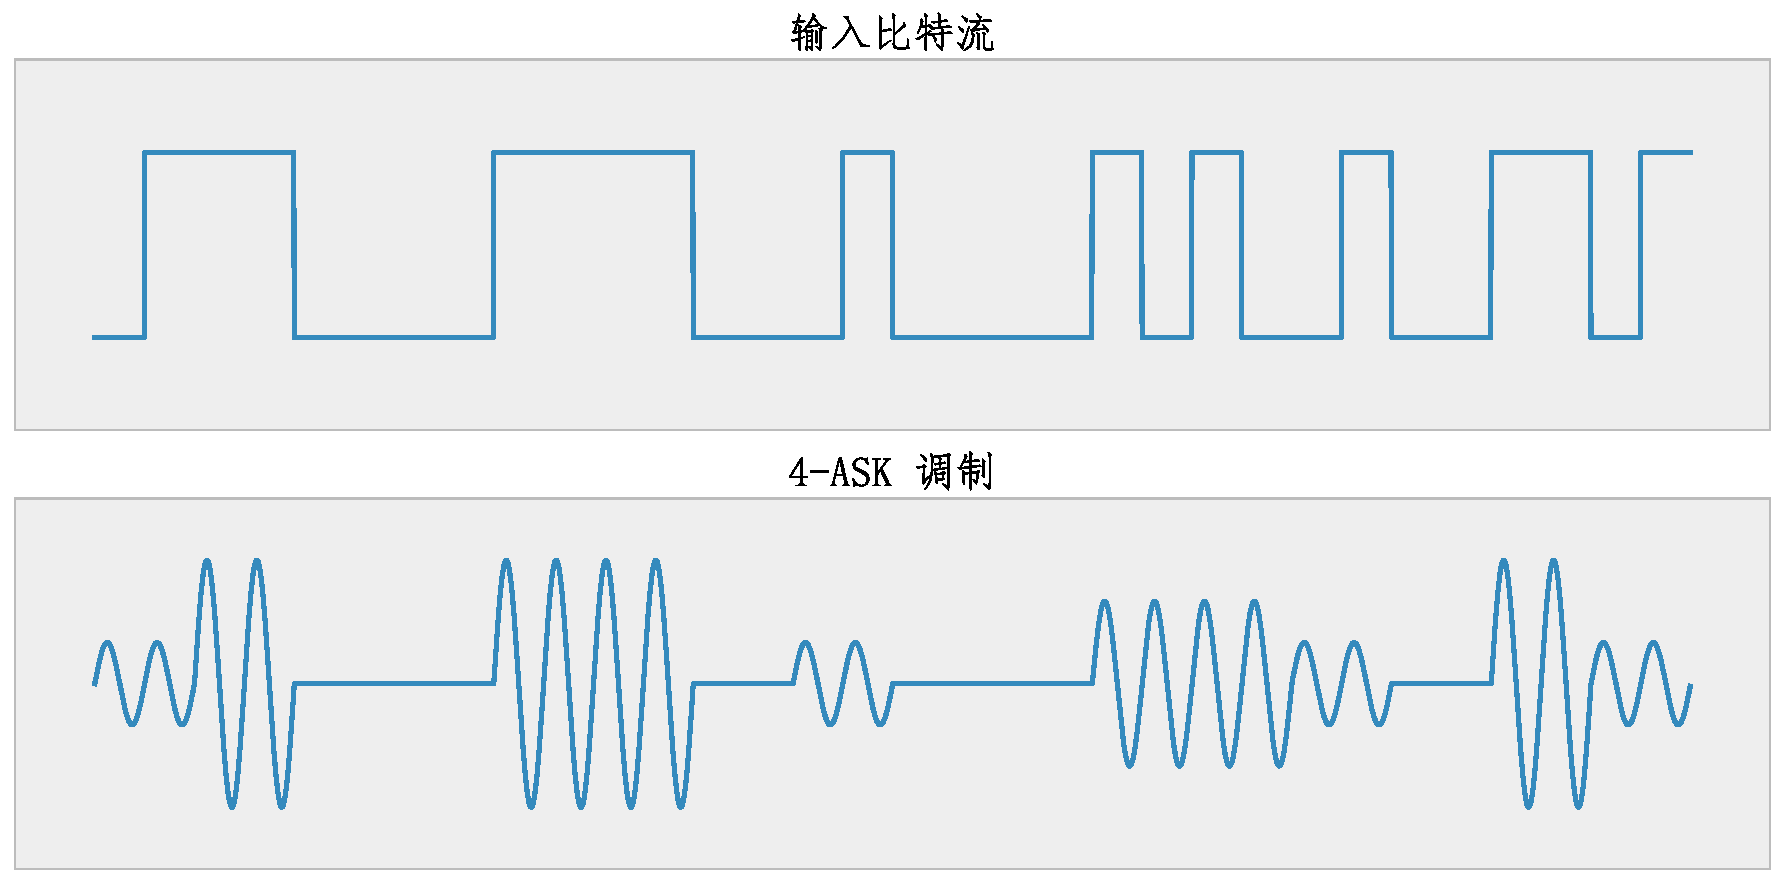
\includegraphics[width=\textwidth]{Image/ask.pdf}
    \caption{幅移键控示意图}
    \label{fig:ASK}
\end{figure}


\subsection{频移键控}\label{sec:background}
% 频移键控是一种将数字信息转换为频率变化的数字调制技术。通常,两个不同的频率代表二进制的0和1。
% \begin{equation}
%     s_{2FSK}(t) = \begin{cases}
%         A \cos(2\pi f_1 t), & a_n = 0 \\
%         A \cos(2\pi f_2 t), & a_n = 1
%     \end{cases}, (n - 1/2)T_b \leq t < nT_b \\
% \end{equation}
% 其中,$A$为信号幅度,$f_1$和$f_2$为信号频率,$T_b$为符号持续时间,$a_n$为比特值。

% 如果要发送数字1,则载波频率切换到一个特定频率;如果要发送数字0,则载波频率切换到另一个特定频率。接收端测量接收到的信号的频率,并根据频率的不同来判断发送的是0还是1。相对于ASK,FSK在噪声环境中表现更好,因为噪声对频率的影响相对较小。

% 多元频移键控(M-ary Frequency Shift Keying,MFSK)可以表示为:
% \begin{equation}
%     s_{MFSK}(t) = Ag(t) \cos(2\pi f_n t), (n - 1) T_s \leq t \leq nT_s
% \end{equation}
% 其中,
% \begin{equation}
%     f_n = f_c + \frac{(2i - M - 1)}{2} \Delta f, i = 0, 1, \dots, M - 1
% \end{equation}
% $f_c$为载波频率,$\Delta f$为频率间隔,$M$为调制阶数。图~\ref{fig:FSK}展示了FSK的示意图。

频移键控(FSK)是一种通过改变载波信号的频率来传输数字信息的调制技术。在FSK中,数字信息(如二进制的0和1)被转换为不同的频率变化。这种调制技术特别适用于需要在噪声环境下传输数据的通信系统,因为相对于幅度变化,频率变化对噪声更具抵抗力。二进制频移键控(2FSK)的数学表达式如下:

% ### 数学表达式
\begin{equation}
    s_{2FSK}(t) = \begin{cases}
        A \cos(2\pi f_1 t), & a_n = 0 \\
        A \cos(2\pi f_2 t), & a_n = 1
    \end{cases}, (n - 1/2)T_b \leq t < nT_b \\
\end{equation}
其中,\( A \) 表示信号幅度,\( f_1 \) 和 \( f_2 \) 分别代表两个不同的频率,\( T_b \) 为比特持续时间,\( a_n \) 为比特值。

在发送数字1时,载波频率切换到 \( f_2 \);相反,发送数字0时,载波频率切换到 \( f_1 \)。接收端通过测量接收信号的频率来确定发送的是0还是1。FSK的主要特点如下:

% ### FSK的特性与应用
抗干扰能力:FSK由于其频率变化特性,在噪声环境中的表现优于幅度变化调制(如ASK),因此在无线通信和数据传输中得到了广泛应用。

功耗:与ASK相比,FSK通常需要更高的带宽,但它提供了更好的信号稳定性和抗干扰能力。

% ### 多元频移键控(MFSK)
MFSK是FSK的一种扩展,它使用多个频率来表示更多的符号,从而提高数据传输速率。
\begin{equation}
    s_{MFSK}(t) = Ag(t) \cos(2\pi f_n t), (n - 1) T_s \leq t \leq nT_s
\end{equation}
其中,
\begin{equation}
    f_n = f_c + \frac{(2i - M - 1)}{2} \Delta f, i = 0, 1, \dots, M - 1
\end{equation}
\( f_c \) 为载波频率,\( \Delta f \) 为频率间隔,\( M \) 为调制阶数。MFSK允许系统在相同的带宽下传输更多的数据,但随着调制阶数的增加,系统的复杂度也会相应提高。

% ### 总结
频移键控因其在噪声环境中的优异表现,以及相对较高的信号稳定性,成为了数字通信中一种重要的调制技术。通过对FSK及其变体MFSK的深入理解,可以更好地把握数字调制过程的特性和应用场景。图~\ref{fig:FSK}所示为频移键控的示意图,展示了不同数字状态下载波频率的变化,直观地反映了FSK调制信号的基本原理和操作方式。

\begin{figure}[htbp]
    \centering
    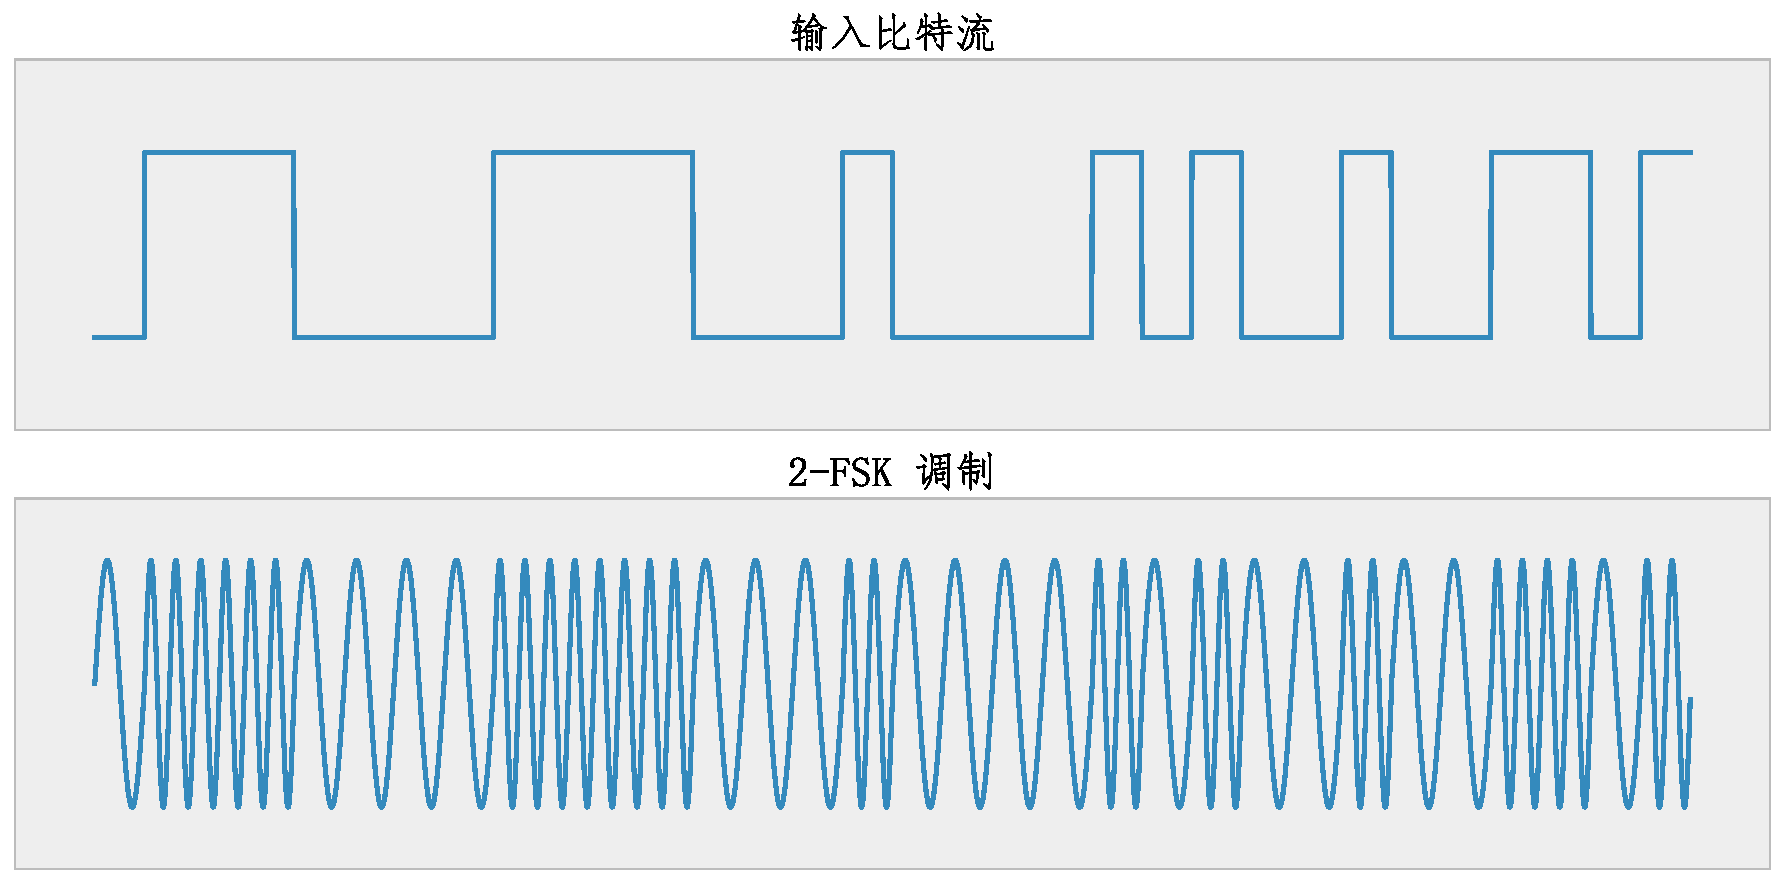
\includegraphics[width=\textwidth]{Image/fsk.pdf}
    \caption{频移键控示意图}
    \label{fig:FSK}
\end{figure}

\subsection{相移键控}\label{sec:background}
% 相移键控中数字信息通过改变载波信号的相位来传递。通常,两个或多个不同的相位表示不同的数字符号。
% \begin{equation}
%     s_{MPSK}(t) = g(t) \cos(2\pi f_c t + \frac{2\pi}{M} (m-1)),
% \end{equation}
% 其中,$g(t)$为基带脉冲成形滤波器,$\theta_m = \frac{2\pi}{M} (m-1)$表示第m个传输符号的载波相位。图~\ref{fig:PSK}展示了PSK的示意图。

% 如果要发送数字1,则载波的相位发生变化到一个特定的角度;如果要发送数字0,则载波的相位发生变化到另一个特定的角度。接收端测量接收到的信号的相位,并根据相位的不同来判断发送的是0还是1。 PSK的带宽效率通常比ASK更高,因为信息通过相位变化而不是振幅变化来传递。PSK在一定程度上对噪声具有抗性,但不如FSK那样抗噪声。PSK相对于ASK和FSK来说更复杂,因为它涉及到相位变化的处理。
相移键控(PSK)是一种将数字信息转换为载波信号相位变化的调制技术。PSK通过改变载波的相位来传输不同的数字符号,通常使用两个或多个不同的相位来表示不同的数字状态。PSK信号的数学表达式如下:

% ### 数学表达式
\begin{equation}
    s_{MPSK}(t) = g(t) \cos(2\pi f_c t + \frac{2\pi}{M} (m-1)),
\end{equation}
其中,\( g(t) \) 是基带脉冲成形滤波器,\( f_c \) 是载波频率,\( \theta_m = \frac{2\pi}{M} (m-1) \) 表示第 \( m \) 个传输符号的载波相位。在二进制PSK中,通常使用两个相位(如0和180度)来表示数字0和1。例如,如果要发送数字1,则载波的相位变化到特定的角度;相反,如果要发送数字0,则载波的相位变化到另一个特定的角度。接收端测量接收到的信号的相位,并根据相位的不同来判断发送的是0还是1。PSK的主要特点如下:

% ### PSK的特性与应用
带宽效率:相对于ASK,PSK具有更高的带宽效率,因为它通过相位变化而不是振幅变化来传递信息。

抗噪声能力:PSK在一定程度上对噪声具有抗性,尤其是在相位同步良好的条件下,但它的抗噪性不如FSK。

复杂性:相对于ASK和FSK,PSK的实现更为复杂,特别是在处理相位变化方面。

% ### 多元相移键控(MPSK)
MPSK是PSK的一种扩展,它使用多个相位来表示更多的符号,从而提高数据传输速率。每个符号通过一个特定的相位来表示,增加了调制的阶数,从而允许更多数据在相同的带宽内传输。

% ### 总结
PSK作为一种重要的数字调制技术,在数字通信中被广泛应用,特别是在需要高带宽效率和适度抗噪声能力的场景。尽管PSK相对于ASK和FSK更为复杂,但它在许多通信系统中因其带宽效率和性能优势而被广泛采用。图~\ref{fig:PSK}所示为相移键控的示意图,清晰展示了PSK调制信号的基本原理,包括如何通过载波的相位变化来表示不同的数字状态。通过对PSK的深入理解,可以更好地掌握数字调制技术的多样性和其在现代通信系统中的应用。

\begin{figure}[htbp]
    \centering
    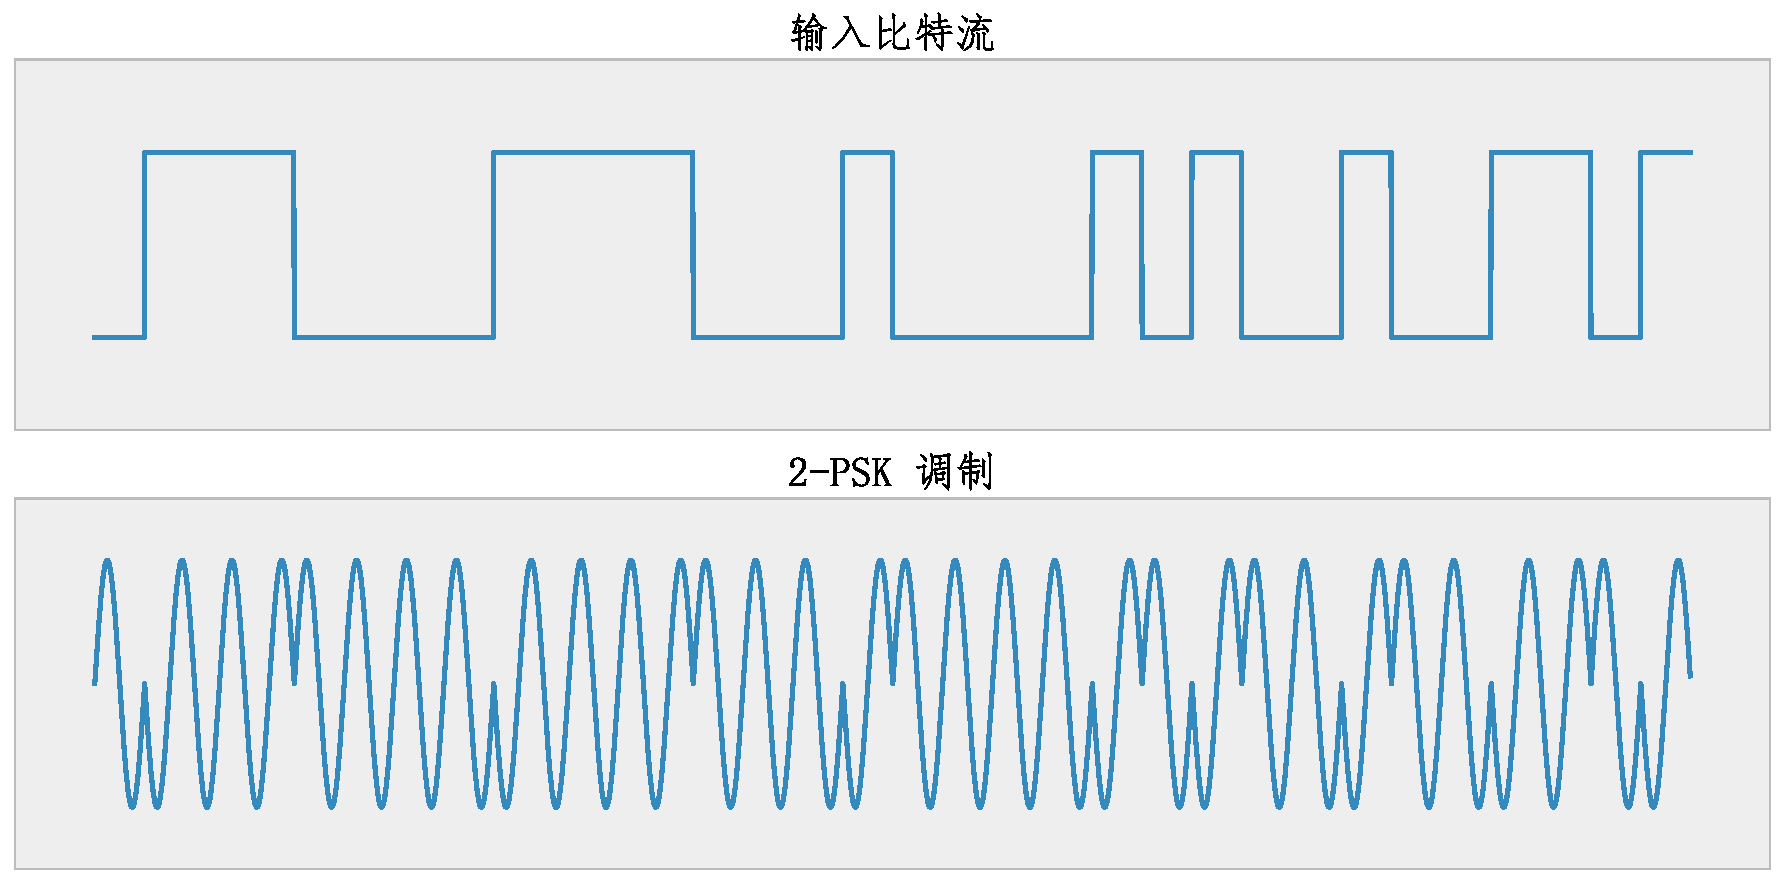
\includegraphics[width=\textwidth]{Image/psk.pdf}
    \caption{相移键控示意图}
    \label{fig:PSK}
\end{figure}


\subsection{正交振幅调制}\label{sec:background}
% 正交振幅调制在信号中同步调制了振幅和相位信息。通常,QAM信号可以表示为在信号空间中的点,其中两个正交的轴分别表示振幅和相位。
% \begin{equation}
%     S_{QAM}(t) = Aa_{cn}g_T(t)\cos(2\pi f_c t) - Aa_{sn}g_T(t)\sin(2\pi f_c t),
% \end{equation}
% 其中,$a_{cn}$和$a_{sn}$分别表示当前传输比特的星座点位置坐标,分别对应了同相支路和正交支路的比特符号。图~\ref{fig:QAM}展示了QAM的示意图。

% QAM通过同时改变振幅和相位来表示数字信息。例如,如果要发送数字11,则信号空间中的点将具有特定的振幅和相位。接收端测量接收到的信号的振幅和相位,并根据这些信息还原发送的数字信息。QAM可以在有限的频谱内传输多个位,因此具有很高的带宽效率。相较于ASK、FSK和PSK,QAM的调制和解调过程更为复杂。
正交振幅调制(QAM)是一种先进的数字调制技术,它通过同时调制信号的振幅和相位来传输数字信息。QAM的独特之处在于它利用信号空间的两个正交维度(即振幅和相位)来表示数据,使得每个符号可以携带更多的信息位。

% ### 数学表达式
QAM信号的数学表达式如下:
\begin{equation}
    S_{QAM}(t) = Aa_{cn}g_T(t)\cos(2\pi f_c t) - Aa_{sn}g_T(t)\sin(2\pi f_c t),
\end{equation}
其中,\( A \) 是载波的振幅,\( g_T(t) \) 是脉冲形状函数,\( f_c \) 是载波频率。\( a_{cn} \) 和 \( a_{sn} \) 分别表示当前传输比特在星座图上的坐标,对应于同相(Inphase)和正交(Quadrature)支路的比特符号。其主要特点如下:

% ### QAM的特性与应用
带宽效率:QAM能够在有限的频谱内传输大量数据,因此具有较高的带宽效率。这使得QAM在需要高数据速率的通信系统中特别有价值。

信号空间:QAM信号可以在信号空间中的点上表示,这些点在两个正交轴上分布,分别代表振幅和相位的不同组合。

复杂性:与ASK、FSK和PSK相比,QAM在调制和解调方面更为复杂。它需要精确的幅相平衡和同步,才能准确地检测信号空间中的点。
抗干扰能力:虽然QAM在抗噪声方面不如某些其他调制方式,但它通过适当的星座图设计和前向纠错编码等技术可以提高抗干扰能力。

% ### 总结
QAM因其高效的带宽利用率在现代通信系统中发挥着重要作用。它通过综合调制振幅和相位,能够在每个符号中携带更多的信息位。尽管QAM的实现相对复杂,但它在高速数据通信领域的应用优势使其成为数字调制技术中的重要组成部分。图~\ref{fig:QAM}所示为正交振幅调制的示意图,展示了QAM信号在信号空间中的表示方式以及如何通过振幅和相位的组合来传输不同的数字信息。通过对QAM技术的深入理解,可以更好地把握数字调制技术的复杂性和其在高数据速率通信系统中的应用。

\begin{figure}
    \centering
    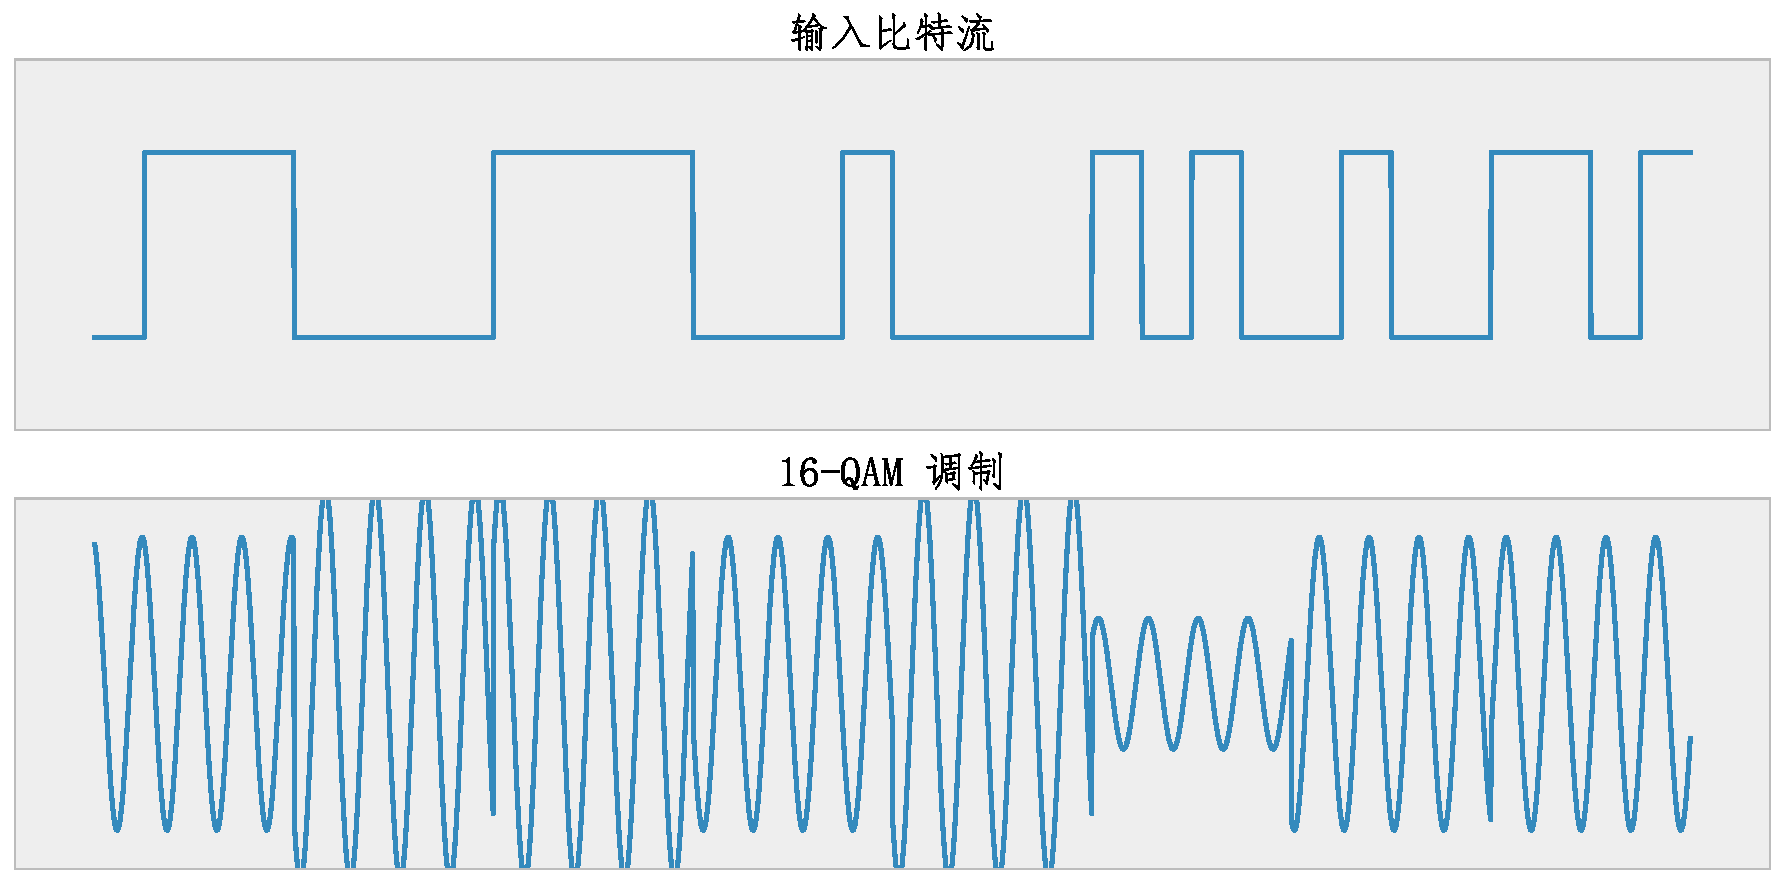
\includegraphics[width=\textwidth]{Image/qam.pdf}
    \caption{正交振幅调制示意图}
    \label{fig:QAM}
\end{figure}

% \dots

% \section{传统方法}\label{sec:background}
% 一般而言,AMR可以看作一种典型的模式识别问题,一般包含三个步骤,接收信号的预处理、特征提取和最后的调制分类。AMR任务的传统方法主要有两类:\textit{基于似然比(Likelihood Based)}的方法\cite{hameed2009likelihood}和\textit{基于特征提取(Feature Based)}的方法~\cite{hazza2013overview}。

% % 虽然基于似然的方法在贝叶斯意义上是最优的,但其通常需要较高的计算复杂性和对于调制信号的先验知识,这使得该方法对未知的信道环境十分敏感,从而影响了其适用性。基于特征提取的方法则受特征选取影响较大,不同的特征其识别结果也有很大的差别,因此如何选取特征 是识别结果好坏的关键。其次,由于特征提取需要花费一定的时间,这就导致了在实际 应用中也难以做到实时处理。~\cite{moser2015automatic}

% \subsection{似然比法}\label{sec:background}
% 基于似然比的方法将AMR视为多重假设检验问题~\cite{xu2010software},对不同的调制类型做出假设,并计算在不同假设下接收信号的似然比。然后,通过将似然比与预定义的阈值进行比较,确定接收信号的调制类型~\cite{dobre2007survey}。
% 似然比法是一种常见的统计方法,用于根据观测到的数据计算不同假设之间的似然比。在自动调制识别中,似然比法通常涉及计算信号的似然比值,然后选择具有最大似然比值的调制方式。当接收端获取到信号后,先对接收信号的未知目标参数进行建模,获取特定参数的概率分布,再根据特定的似然准则建立似然函数,计算每一个假设调制方式类型对应的似然值,最后根据贝叶斯信息准则(Bayesian Information Criterion, BIC),在一定阈值的约束下,选取最大似然值所对应的调制方式作为目标信号的预测调制方式。图~\ref{fig:likelihood}展示了似然比假设检验识别法的处理流程。

% \begin{figure}
%     \centering
%     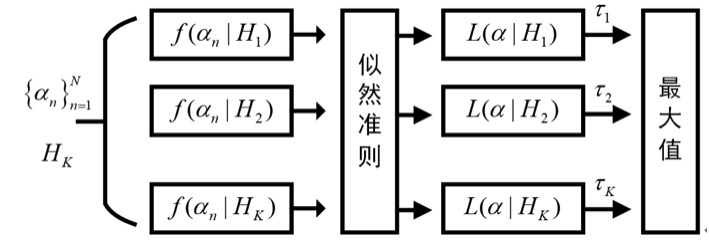
\includegraphics[width=0.8\textwidth]{Image/lb.jpg}
%     \caption{似然比法处理流程}
%     \label{fig:likelihood}
% \end{figure}
% 似然比法的不足:

% 对于复杂的信号模型,需要准确的先验知识,且在高维度空间中可能难以处理。

% 对噪声和非理想条件敏感,容易受到信噪比的影响。

% \dots

% \subsection{特征提取法}\label{sec:background}
% 特征提取法通过从信号中提取相关特征,如能量、频率分布和相位信息等,然后利用这些特征进行调制识别。其整个识别流程一般包括三个步骤,即信号预处理、特征提取和分类器识别,其中特征提取是关键步骤。信号预处理旨在通过对信号进行简单的变换,使其具有一定规范性,以降低后续数据处理的难度,例如对接收信号进行滤波和降频处理。同时,也需要对信号数据进行清洗和筛选,排除不合理的数据信息。特征提取的任务是在不同维度中寻找各种调制方式之间的差异。对于同一种调制方式,不同的特征反映出的调制信息也具有显著差异,其识别结果也存在一定的差异。因此,相较于基于统计模式的识别算法,选取适当的特征对于提高识别精度至关重要。图~\ref{fig:feature}展示了调制识别领域中常用的信号维度特征。

% \begin{figure}
%     \centering
%     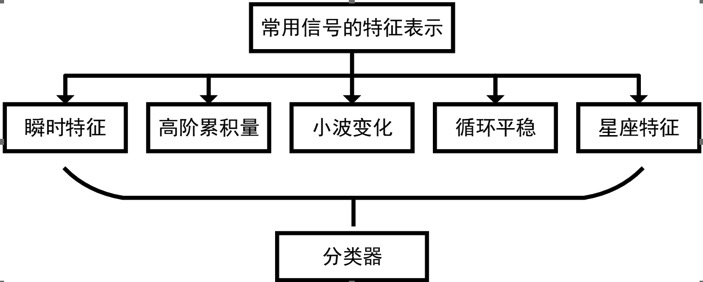
\includegraphics[width=0.8\textwidth]{Image/fb.jpg}
%     \caption{常用的信号维度特征}
%     \label{fig:feature}
% \end{figure}
% 特征提取法的不足:

% 依赖于手动设计的特征,可能无法适应复杂信号模式的变化。

% 难以处理大规模数据,且对特征选择的依赖可能导致信息丢失。

% \dot


\section{调制识别方法原理}\label{sec:background}

在自动调制识别领域,传统方法的研究进展主要集中在利用经典的信号处理技术和决策理论。这些方法通常依赖于从接收信号中提取特定的统计特征,如瞬时幅度、相位和频率等,来识别信号的调制类型。这些传统方法包括决策树、支持向量机(SVM)和人工神经网络等,它们在高信噪比(SNR)环境下能够实现较高的识别准确率。然而,这些方法在复杂的通信环境,如低信噪比或多径衰落条件下,性能往往受到限制。

传统的AMR方法主要依赖于特定的统计特征和经典的信号处理技术。这些方法在信噪比较高、环境相对稳定的情况下表现良好。然而,它们在处理复杂或低信噪比信号时的性能往往不足,且通常需要复杂的特征提取和大量的先验知识。
接下来介绍下似然比法的基本原理:

似然比法是一种经典的传统方法,长期以来一直是研究者们的关注焦点。似然比法基于统计决策理论,通过计算接收到的信号数据在不同假设调制类型下的似然比来实现调制类型的识别。这种方法的核心是利用接收信号的统计特性,结合已知调制类型的概率模型,估计信号的调制类型。

似然比法的工作原理建立在贝叶斯理论的基础上。该方法假设对于每一种可能的调制类型,信号都有一个相应的概率模型。这些概率模型描述了在特定调制类型下接收信号的统计特性。在实际应用中,似然比法通过计算每种调制类型下信号观测值的条件概率密度函数,并将其进行比较,从而确定最可能的调制类型。这一过程涉及到复杂的概率计算,尤其是在面对多种调制类型和大量数据时。

实施似然比法的过程主要包含以下几个步骤:首先,对于每一种可能的调制类型,建立一个相应的概率模型,通常是条件概率密度函数。然后,对于接收到的每个信号样本,计算在各种调制假设下的似然比。最后,选择具有最大似然比的调制类型作为识别结果。

似然比法在自动调制识别(AMR)中使用的核心公式是基于计算给定观测数据下不同调制类型的似然比。以下是似然比法中常用的一些基本公式及其简单介绍:

1. 似然函数:
    对于给定的观测数据 \( \mathbf{x} \) 和假设的调制类型 \( M \),似然函数定义为 \( L(\mathbf{x} | M) \),表示在调制类型 \( M \) 下观测到 \( \mathbf{x} \) 的概率。
\begin{align}
    L(\mathbf{x} | M) = p(\mathbf{x} | M),
\end{align}
    % \[ L(\mathbf{x} | M) = p(\mathbf{x} | M) \],
     其中 \( p(\mathbf{x} | M) \) 是在调制类型 \( M \) 下观测数据 \( \mathbf{x} \) 的条件概率密度函数。

2. 似然比:
   似然比是两种调制类型下似然函数的比值。对于两种假设的调制类型 \( M_1 \) 和 \( M_2 \),似然比定义为两者似然函数的比率。
\begin{align}
    \Lambda(\mathbf{x}) = \frac{L(\mathbf{x} | M_1)}{L(\mathbf{x} | M_2)},
\end{align}
%    \[ \Lambda(\mathbf{x}) = \frac{L(\mathbf{x} | M_1)}{L(\mathbf{x} | M_2)} \],
     这里 \( \Lambda(\mathbf{x}) \) 是似然比,用于比较两种调制类型的可能性。

3. 决策规则:
   在似然比法中,通过比较似然比与预先设定的阈值来做出决策。如果似然比超过阈值,选择一种调制类型;否则,选择另一种。
   如果 \( \Lambda(\mathbf{x}) > \text{阈值} \),选择 \( M_1 \);否则选择 \( M_2 \)。

似然比法的关键在于准确地估计条件概率密度函数 \( p(\mathbf{x} | M) \)。这通常涉及对信号模型的深入理解和复杂的数学运算。在实际应用中,由于通信信号的多样性和复杂性,这些概率密度函数的准确估计是似然比法中最具挑战性的部分。

似然比法在理想条件下能提供较高的识别准确率,这是因为它直接利用了信号的统计特性,并结合了精确的数学模型。这种方法在理论上具有坚实的基础,能够在信号质量良好时实现精确的调制类型识别。

然而,似然比法在实际应用中也存在一些明显的限制。最主要的挑战之一是计算复杂度高。由于需要进行大量的概率计算,特别是在多种调制类型和大数据量的情况下,这一方法的计算成本非常高。此外,似然比法对信噪比(SNR)非常敏感。在低信噪比或非理想信道条件下,其性能可能会显著下降。此外,该方法的性能依赖于对信号模型的精确知识,对模型假设的不准确可能导致识别性能下降。

尽管似然比法在理论上具有优势,并且在理想条件下可以实现较高的识别准确率,但它在实际应用中面临诸多挑战。这些挑战包括高计算复杂度、对低信噪比情况的敏感性以及对精确模型假设的依赖。因此,在现代通信系统中,研究者们开始探索其他方法,特别是那些能够更有效地处理复杂信号环境和大数据量的方法,如基于深度学习的AMR技术。随着计算能力的提升和算法的发展,深度学习方法在AMR领域显示出巨大的潜力,逐渐成为研究的新热点。尽管如此,似然比法作为一种经典的方法,在理论研究和特定应用场景中仍然具有重要价值。

特征提取方法是另一种常用的传统AMR方法。与似然比法不同,特征提取方法不直接利用信号的统计特性,而是通过从信号中提取特征来实现调制类型的识别。特征提取方法通常包含两个基本步骤:特征的选择和分类器的设计。特征选择的目的是从信号中提取最具代表性的特征,以实现最佳的识别性能。分类器的设计是为了将提取的特征与预先定义的调制类型进行匹配,从而实现调制类型的识别。

接下来将从信号特征的表示和分类器的设计两个方面介绍特征提取方法。

\textbf{(一)信号特征的表示}

1. 瞬时特征:
   瞬时幅度、相位和频率是分析调制信号中最基本的特征。瞬时幅度反映了信号强度的即时变化,瞬时相位提供了关于信号相位变化的信息,而瞬时频率揭示了信号频率随时间的变化情况。这些特征对于区分例如ASK(幅度键控)、FSK(频率键控)和PSK(相位键控)等基本调制类型非常有效。

2. 高阶统计特征:
   这类特征包括偏度和峰度,用于分析信号的分布形状和尾部特性。例如,高阶累积量如二阶和四阶矩可用于捕捉信号的非高斯特性。这些高阶统计特征对于识别复杂调制模式,如QAM(正交幅度调制)特别有用。

3. 变换域特征:
   变换域特征涉及将时间域信号转换到频域或其他域,例如通过傅里叶变换或小波变换。频域特征有助于理解信号的频率组成,特别是在频域中能量分布的特点。这对于识别频谱利用率和频谱效率高的调制类型尤为重要。

4. 星座图特征:
   星座图是调制信号在复平面上的图形表示,它为调制过程提供了直观的视图。通过分析星座图的形状、密度和分布,可以提取关于调制类型的重要信息。例如,不同的QAM调制在星座图上呈现不同的点分布模式。

5. 时频分布特征:
   时频分布特征提供了信号随时间变化的频率特性,适合于分析非平稳信号。通过分析时频分布,可以识别具有时间变化特性的复杂调制信号,这在现代通信系统中尤为重要。

\textbf{(二)分类器}

1. 支持向量机(Support Vector Machine, SVM):
   SVM是一种有效的分类算法,通过在特征空间中寻找最佳分割超平面来区分不同类别的数据。SVM特别适用于具有明显边界的分类问题。在AMR中,SVM可用于区分具有不同特征向量的调制类型。

2. 决策树:
   决策树通过从根到叶的顺序决策过程对数据进行分类。每个节点代表一个特征的决策点,根据该特征的值选择分支,直到到达叶节点,即分类结果。决策树易于理解和实现,适用于具有明显特征规则的调制类型识别。

3. 随机森林:
   随机森林是基于多个决策树构建的集成学习方法。它通过组合多个树的预测结果来提高分类的准确性和鲁棒性。在AMR中,随机森林能够有效处理大量的特征并提供稳定的分类结果。

4. 神经网络:
   神经网络,尤其是浅层神经网络,可用于特征提取法中的分类任务。它们通过学习特征与调制类型之间的非线性关系来进行分类。神经网络在处理复杂的调制识别问题时表现出色,尤其是当特征空间维度较高时。

5. K最近邻(K-Nearest Neighbor, KNN):
   KNN是一种基于邻近样本进行分类的简单方法。它根据最近邻样本的类别来决定新样本的类别。虽然KNN在小规模数据集上效果良好,但在大数据集上的计算成本较高。

特征提取法在AMR中的应用表明,有效的特征提取和精准的分类是提高调制识别性能的关键。随着通信技术的发展,尤其是在面对更复杂的信号和通信环境时,对于更先进的特征提取技术和更有效的分类算法的需求日益增长。

\subsection{传统方法的局限性}\label{sec:background}

在自动调制识别(AMR)的研究中,传统方法虽然在特定情况下表现良好,但它们也存在一些显著的缺陷,这限制了它们在复杂通信环境中的应用。这些局限性包括:

高计算复杂度:传统的AMR方法,特别是似然比法,涉及复杂的数学运算和概率计算,尤其是在多种调制类型和大数据量的情况下。这种高计算复杂度限制了其在实时或资源受限的应用中的可行性。

模型失配问题:传统方法往往依赖于对信号模型的精确假设。然而,在实际应用中,由于信道效应、噪声以及硬件限制等因素,实际信号可能与理论模型存在差异,导致模型失配。这种失配会显著降低识别准确率。

对特征提取的依赖:特征提取法的性能在很大程度上依赖于所选特征的有效性。不恰当或不充分的特征提取可能导致分类性能下降。此外,手动特征工程是一个复杂且耗时的过程,对先验知识和专业判断的依赖较大。

对信噪比的敏感性:在低信噪比或非理想信道条件下,传统AMR方法的性能可能会显著下降。这些方法对信号质量的依赖性限制了它们在复杂通信环境下的应用。

\subsection{深度学习方法}\label{sec:background}
近年来,深度学习技术为AMR带来了革命性的改变。深度学习模型,特别是卷积神经网络(Convolution Neural Network, CNN)和循环神经网络(Recurrent Neural Network, RNN),已经被证明在从原始信号中直接提取特征和执行复杂的分类任务方面非常有效。这些模型能够在多种条件下实现高准确率的调制识别,即使在低信噪比或非理想信道条件下也是如此。尽管如此,深度学习方法在处理AMR问题时仍面临诸如训练数据需求量大、模型复杂度高以及对低信噪比情况下性能的提升等挑战。接下来将详细介绍主要的深度学习模块及其在调制识别问题中的优势:

1.卷积神经网络(CNN)是深度学习中的基础模型之一,特别适用于处理具有空间结构的数据。CNN通过其多层卷积结构能够从原始I/Q数据中自动提取特征,无需复杂的特征工程。CNN的每一层都能捕获信号的不同层次特征,而池化层则用于降低特征的维度和复杂性,增强模型的泛化能力。在调制识别中,CNN的主要优势在于其强大的特征提取能力,使其能够适应不同的调制类型,即使在低信噪比环境下也能保持较好的性能。

2.循环神经网络(RNN)和长短期记忆网络(LSTM)是处理时间序列数据的理想选择,能够有效捕捉数据中的时间依赖性。RNN通过其循环结构捕获时间序列中的信息,适用于处理时间相关的信号特性。LSTM引入了遗忘门和输入门,能够有效地处理长期依赖问题,避免了RNN中的梯度消失问题。在AMR中,RNN/LSTM的优势在于它们能够处理信号的时序特征,尤其适用于识别那些具有复杂时间结构的调制类型。

3.注意力机制是一种使模型能够聚焦于输入数据中最重要部分的技术,能够提高模型对关键信息的敏感性。注意力机制使模型能够识别并集中处理输入数据的关键部分,提高处理效率和准确性。在调制识别应用中,注意力机制尤其有用于识别那些在特定时间窗口或频率范围内具有显著特征的信号类型。它能够帮助模型集中处理最关键的信号部分,提高识别准确率。

总体而言,深度学习方法为AMR提供了一种高效且强大的替代方案。这些方法能够直接从原始信号中自动提取特征,并有效地处理各种调制类型。CNN的特征提取能力、RNN/LSTM的时间依赖性处理能力以及注意力机制的关键信息聚焦能力,使它们在处理复杂的调制识别问题时表现出色。随着技术的不断发展,深度学习方法有望在AMR领域中发挥越来越重要的作用,特别是在应对复杂通信环境和高动态信号条件下的挑战。

\subsubsection{宽带信号调制识别}\label{sec:background}

宽带信号调制识别在自动调制识别领域中呈现出独特的挑战,主要由于其涉及的频率范围广泛且信号特性复杂。从采样角度来看,宽带信号的处理面临着存储和设备成本的重大挑战。传统的采样方法按照奈奎斯特定理要求,采样频率必须至少是信号最高频率的两倍,这在宽带信号的情况下导致了极高的采样率。高采样率随之带来的数据量巨大,不仅需要大量存储空间,而且对数据处理提出了高要求,增加了数据处理的复杂性。此外,实现这种高速采样的设备往往昂贵,限制了宽带信号处理技术的普及。

为了克服这些挑战,亚采样(本研究中选取多陪集采样)技术应运而生。亚采样技术允许以低于奈奎斯特速率的采样频率对信号进行采样,从而减少了所需的存储空间和处理能力,降低了设备成本。通过采用特定的采样策略和后续的信号处理算法,可以从低速率采样的数据中恢复出原始信号的关键信息。

在宽带信号识别方面,自动调制识别的研究相对较少,但随着宽带通信技术的发展,对于这方面的研究需求正在迅速增长。在宽带信号的处理中,自动调制识别不仅需要识别信号的调制类型,还需要确定信号占用的子带位置。这增加了自动调制识别的复杂性,因为宽带信号涉及更广泛的频率范围和更复杂的信号特性。亚采样技术在这里发挥着关键作用,它通过降低采样率,使得对宽带信号的处理变得更为可行和经济。

然而,亚采样技术也带来了新的挑战,尤其是在信号重构和调制类型识别方面。如何从低速率采样的数据中准确地恢复出信号的关键特征,并进行有效的调制识别,是当前研究的重点。这需要创新的信号处理算法和先进的数据分析技术,以从有限的采样数据中提取出足够的信息进行准确的调制识别。

目前,针对宽带信号的自动调制识别技术仍处于发展阶段,需要更多的研究来解决宽带环境下的特定挑战,特别是在信号重构和调制类型识别的准确性方面。未来的研究可能会集中在开发新的亚采样技术和相关的信号处理算法,以提高宽带信号处理的效率和准确性。同时,随着深度学习等先进技术的应用,有望在提高宽带信号自动调制识别性能方面取得重要进展。

总体而言,自动调制识别领域的研究正在从传统方法向深度学习方法转变,每种方法都有其独特的优势和局限性。随着通信技术的不断发展,特别是宽带通信技术的兴起,自动调制识别技术面临着新的挑战和机遇。未来的研究需要关注在复杂环境下提高自动调制识别性能的方法,尤其是在处理宽带信号方面的进展和挑战。


\section{深度学习理论基础}\label{sec:background}

神经网络的基本结构由输入层、隐藏层和输出层构成,它们通过带权重的连接相互作用。在深度学习中,这些层可以堆叠起来形成深度神经网络,以学习输入数据中的复杂模式和特征。每一层都由若干神经元组成,其中每个神经元负责对输入数据进行一定的数学变换。这些变换通常涉及到权重(\(W\))和偏置(\(b\))的线性组合,随后通过一个非线性的激活函数(\(f\))进行处理。这种结构使得神经网络能够逼近几乎任何复杂的函数。
神经网络由多层神经元组成,每层神经元可以接收上一层神经元的输出作为输入,并产生输出到下一层。一个基本的三层神经网络可以表示为:

\begin{equation}
    y = f(W_2 f(W_1 x + b_1) + b_2)
\end{equation}

其中,\( x \) 是输入向量,\( W_1 \) 和 \( W_2 \) 是权重矩阵,\( b_1 \) 和 \( b_2 \) 是偏置向量,\( f \) 是激活函数,\( y \) 是输出向量。在这种结构中,\( W_1 \) 和 \( b_1 \) 对应于第一层(通常称为隐藏层)的权重和偏置,而 \( W_2 \) 和 \( b_2 \) 对应于第二层(输出层)的权重和偏置。激活函数 \( f \) 用于引入非线性,使得网络能够学习和模拟非线性关系。

每一层的神经元数量和层的总数可以根据特定的应用和数据集进行调整。隐藏层的深度和宽度(即每层的神经元数量)是神经网络设计中的关键参数,它们直接影响到网络的能力和复杂度。理论上,增加更多的隐藏层和神经元可以使网络能够学习更复杂的函数,但这也会增加训练的难度和过拟合的风险。

在训练过程中,通过反向传播算法和梯度下降等优化方法调整权重和偏置,以最小化网络输出和真实标签之间的差异。这个过程涉及到计算损失函数(如均方误差或交叉熵损失)相对于网络参数的梯度,并根据这些梯度更新参数。

神经网络的这种层级结构和训练机制使其成为一种强大的工具,能够应用于广泛的任务,包括图像识别、语音识别、自然语言处理等领域。通过调整网络结构和参数,研究人员和工程师能够设计出适应特定问题的模型,解决传统算法难以处理的复杂任务。

\subsection{激活函数}\label{sec:background}
激活函数用于引入非线性,使得神经网络可以学习并表示复杂的函数。常见的激活函数包括:

\subsubsection{Sigmoid函数}
Sigmoid函数是一个常用的激活函数,它的数学表达式如公式\ref{eq:sigmoid}所示:
\begin{equation}
    \sigma(x) = \frac{1}{1 + e^{-x}}
    \label{eq:sigmoid}
\end{equation}
\begin{figure}
    \centering
    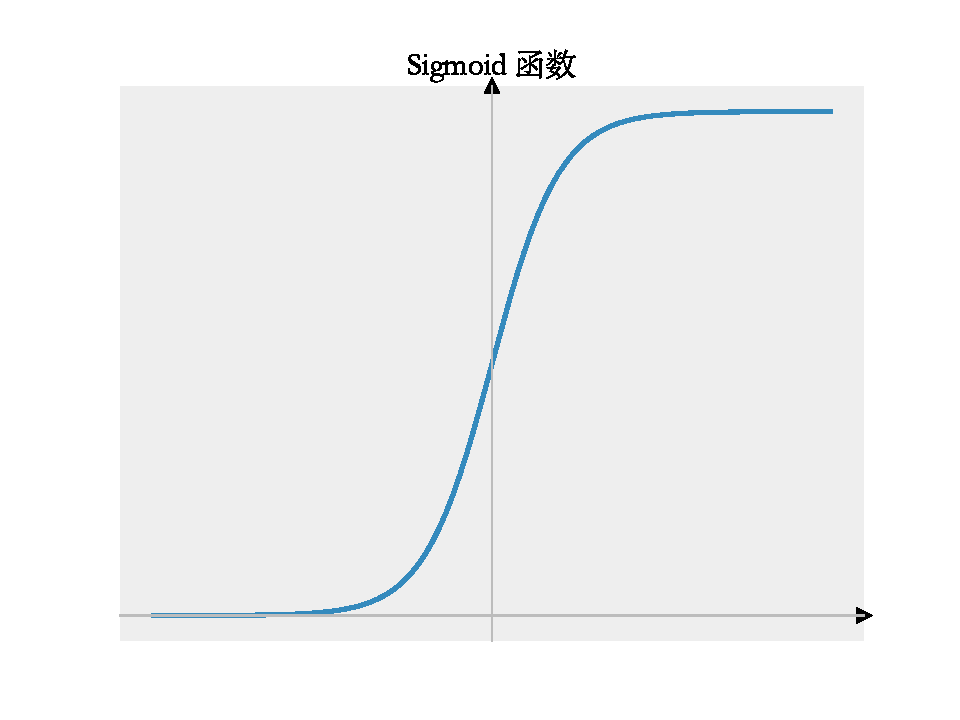
\includegraphics[width=0.8\textwidth]{Image/sigmoid.pdf}
    \caption{Sigmoid函数}
    \label{fig:sigmoid}
\end{figure}

Sigmoid函数是一个在机器学习和深度学习领域广泛应用的非线性函数。其特征在于将任意实数值映射到(0, 1)区间内,使其能够表示概率、进行二分类等。函数图形呈S形曲线,如图像\ref{fig:sigmoid}所示,因而得名Sigmoid(即“S形”的意思)。

Sigmoid函数的取值范围限定在(0, 1)之间,这一性质使其尤为适用于需要输出概率预测的场合,如二分类问题的概率输出。数学上,当输入值x趋向于正无穷时,\( \sigma(x) \)趋近于1;当x趋向于负无穷时,\( \sigma(x) \)趋近于0。正是由于这种平滑的过渡特性,Sigmoid函数能够在模型中充当激活函数,将线性输入转换为非线性输出,为神经网络模型提供必要的非线性特性,使得网络能够学习和模拟复杂的函数映射关系。

然而,Sigmoid函数也存在一些局限性,如梯度消失问题,即当输入值处于饱和区(即极大或极小值附近)时,其梯度接近于零,导致在这些区域内,参数更新缓慢,影响模型的学习效率。尽管如此,由于其形式简单、易于理解,Sigmoid函数在早期的神经网络研究中扮演了重要角色,并为后续的激活函数设计提供了基础。


\subsubsection{ReLU函数}
ReLU(Rectified Linear Unit,修正线性单元)函数是一种在深度学习模型中广泛使用的激活函数,数学表达式如公式\ref{eq:relu}所示:
\begin{equation}
    \text{ReLU}(x) = \max(0, x)
    \label{eq:relu}
\end{equation}
\begin{figure}
    \centering
    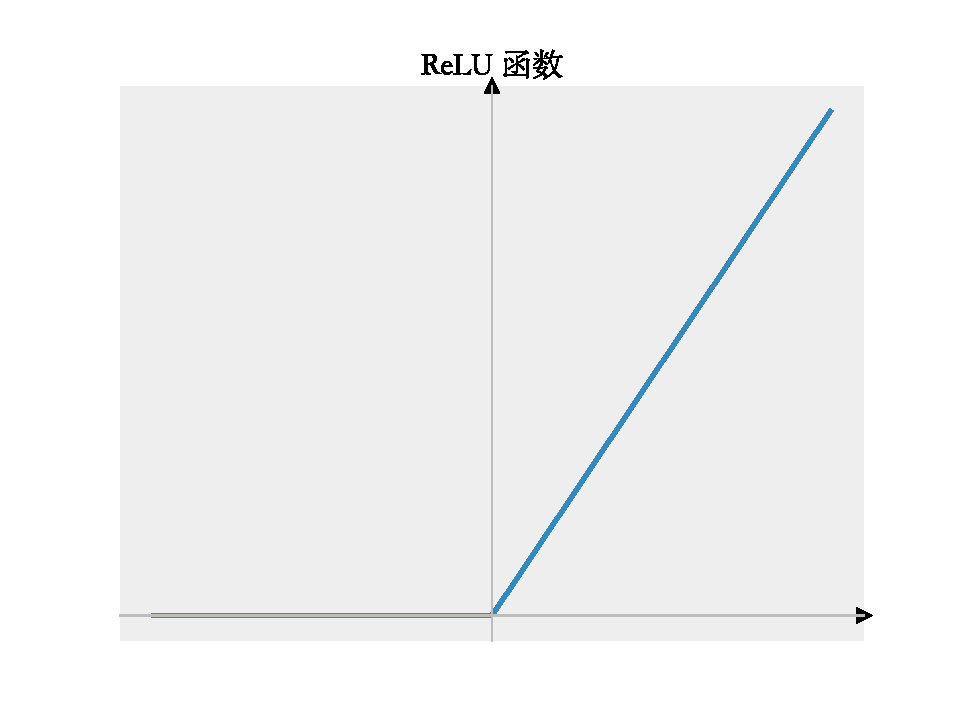
\includegraphics[width=0.8\textwidth]{Image/relu.pdf}
    \caption{ReLU函数}
    \label{fig:relu}
\end{figure}

该函数的特点是对于所有正数输入保持线性,而对于负数输入则输出为零。ReLU函数的图形表现为一个折线,如图像\ref{fig:relu}所示,其中$x>0$时,函数输出等于输入;$x≤0$时,输出恒为0。

ReLU函数因其计算简单、梯度传播效率高而受到广泛欢迎。在正数区域,ReLU的梯度恒为1,这一性质有利于减轻深度神经网络训练过程中的梯度消失问题,相比之下,Sigmoid函数和Tanh函数在输入值绝对值较大时梯度接近于零,容易引发梯度消失问题。此外,ReLU激活函数还能够通过其非饱和的性质促进神经网络中稀疏激活的产生,有助于提高网络的表达能力和计算效率。

然而,ReLU函数也有其局限性,其中最著名的是“死亡ReLU”问题。这是指在网络训练过程中,一旦某个神经元的输入在训练过程中始终为负数,则该神经元的输出始终为0,导致相应参数不再更新,这样的神经元被称为“死亡”神经元。为了克服这一问题,研究人员提出了多种ReLU的变体,如Leaky ReLU、Parametric ReLU等,这些变体试图保留ReLU在正区间的线性特性,同时为负区间的输入提供一个小的、非零的梯度,以促进全面的参数更新。

尽管存在上述问题,但得益于其简洁性和效率,ReLU及其变体仍然是当前深度学习领域最为流行和有效的激活函数之一。

\subsubsection{Tanh函数}
Tanh(双曲正切)函数是一种常用的激活函数,其数学表达式如公式\ref{eq:tanh}所示:
\begin{equation}
    \tanh(x) = \frac{e^x - e^{-x}}{e^x + e^{-x}}
    \label{eq:tanh}
\end{equation}
\begin{figure}
    \centering
    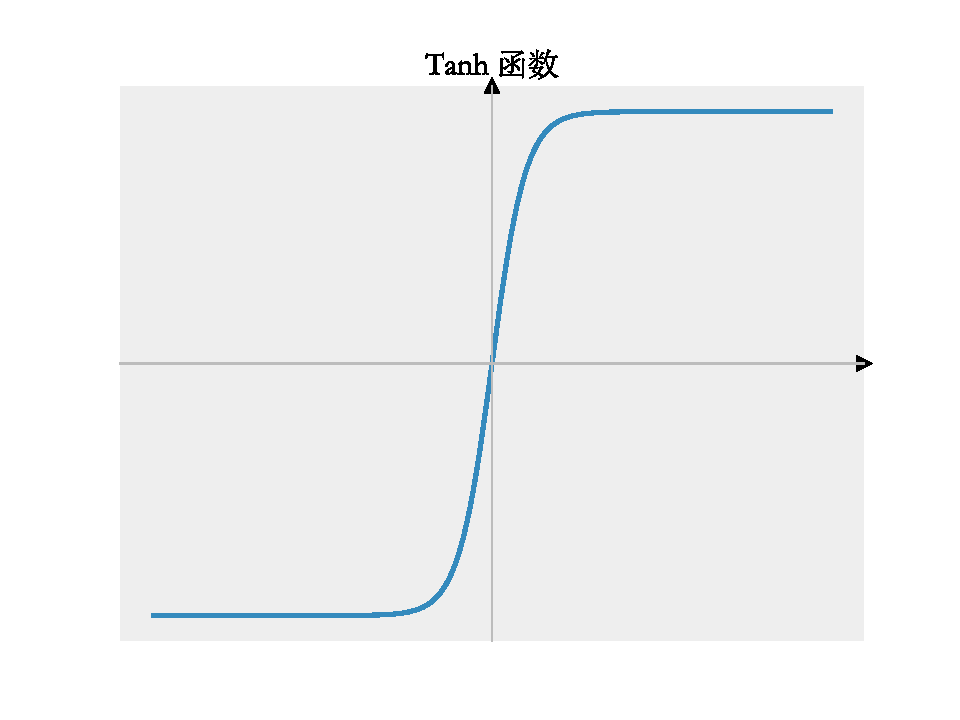
\includegraphics[width=0.8\textwidth]{Image/tanh.pdf}
    \caption{Tanh函数}
    \label{fig:tanh}
\end{figure}
与Sigmoid函数类似,Tanh函数也是一种S形的非线性激活函数,如图\ref{fig:tanh}所示,但其输出范围是(-1, 1),这一点与Sigmoid函数的输出范围(0, 1)有所不同。Tanh函数在输入值为0时输出0,其对称性有助于数据的中心化,这通常能够加快收敛速度,改善学习效率。

Tanh函数的主要优点之一是其输出范围,因为它能够输出负值,所以在处理以0为中心的数据时比Sigmoid函数表现更好。这种以0为中心的性质使得Tanh函数在一些场合下比Sigmoid函数更受青睐,特别是在隐藏层的激活函数选择上。在神经网络的训练过程中,Tanh函数能够有效地控制正向和反向传播时梯度的大小,从而避免了Sigmoid函数中可能出现的梯度消失问题。

然而,尽管Tanh函数比Sigmoid函数具有更好的性能,它仍然不能完全避免梯度消失的问题,特别是在处理深层网络时。当输入的绝对值很大时,Tanh函数的梯度也会接近于零,这会导致深层网络在训练过程中更新速度缓慢。

尽管存在这些局限性,Tanh函数由于其输出范围和性能,依然是深度学习领域中常用的激活函数之一,尤其适用于要求输出为双向的场合,如一些特定的神经网络架构中。随着深度学习领域的发展,Tanh函数和其他激活函数一样,根据特定的应用场景和网络架构被灵活选用,以达到最优的模型性能。

\subsection{反向传播算法}\label{sec:background}
反向传播算法是深度学习中最核心的概念之一,它允许网络通过梯度下降法高效地调整其参数,以最小化损失函数。这一过程涉及到对网络中每一层逐层反向计算梯度,并根据这些梯度更新相应的参数。对于一个简单的两层网络,参数更新可以表示为:

\begin{equation}
    W = W - \eta \frac{\partial \mathcal{L}}{\partial W}
\end{equation}

其中,\(W\) 是权重矩阵,\(\eta\) 是学习率,\(\mathcal{L}\) 是损失函数。

深度神经网络的训练分为两个阶段:前向传播和反向传播。在前向传播阶段,输入数据沿着网络前进,通过每一层的加权和及激活函数处理,最终产生输出。这一过程中,每一层的输入和输出都被存储起来,以便之后的梯度计算。

在反向传播阶段,算法从输出层开始,逆向通过网络,计算每一层的梯度。这一过程利用链式法则,根据损失函数相对于网络参数的偏导数来计算梯度。具体来说,对于每一层,损失函数的梯度可以表示为该层输出对损失的影响和该层输入对其输出的影响的乘积。

梯度计算完成后,参数更新规则被用来调整网络中的权重和偏置,以减少预测值和实际值之间的差异。这一更新过程可以通过多种优化算法来实现,如随机梯度下降(SGD)、Adam或RMSprop等。

反向传播算法的成功部分在于其能够有效地计算网络中所有参数的梯度,即使在网络结构非常复杂时也是如此。这使得神经网络能够通过学习过程自动调整其参数,从而在各种任务中实现优秀的性能。此外,反向传播算法的效率和普适性使其成为训练深度学习模型的基石之一。
\subsection{损失函数}\label{sec:background}
损失函数在神经网络中扮演着至关重要的角色,它量化了模型输出与真实标签之间的差异。选择合适的损失函数对于训练有效的神经网络模型是非常关键的。常见的损失函数有均方误差(MSE)和交叉熵损失,它们分别适用于回归问题和分类问题。

\subsubsection{均方误差(MSE)} 
均方误差是最常用的回归损失函数,定义为预测值与真实值之差的平方和的平均值。数学表达式为:
\begin{equation}
    \mathcal{L}_{\text{MSE}} = \frac{1}{n} \sum_{i=1}^{n} (y_{\text{pred}, i} - y_{\text{true}, i})^2
\end{equation}
其中,\(y_{\text{pred}, i}\) 是第\(i\)个样本的预测值,\(y_{\text{true}, i}\) 是对应的真实值,\(n\) 是样本总数。

\subsubsection{交叉熵损失(Cross-Entropy Loss)}
交叉熵损失是处理分类问题时最常用的损失函数之一,特别是在二分类和多类分类问题中。它衡量的是实际输出的概率分布与预测输出的概率分布之间的差异。对于二分类问题,交叉熵损失的数学表达式为:
\begin{equation}
    \mathcal{L}_{\text{CE}} = -\sum_{i=1}^{n} [y_{\text{true}, i} \log(y_{\text{pred}, i}) + (1 - y_{\text{true}, i}) \log(1 - y_{\text{pred}, i})]
\end{equation}
对于多类分类问题,其表达式稍有不同,但核心概念保持一致,即最小化真实标签和预测概率之间的差异。

通过精心设计的损失函数,可以引导神经网络在训练过程中不断调整参数,以期望输出更接近于真实标签。损失函数的选择依赖于特定的任务(如回归或分类)和所需的性能指标。


\section{宽带信号模型}\label{sec:background}


宽带信号的模型是现代通信系统中一个重要的概念,其特点是包含多个子带信号,这些子带信号经过不同频率的频移后叠加在一起。下面是对宽带信号模型的数学表述及其关键假设的进一步阐述。

\subsection{宽带信号的数学模型}\label{sec:background}
宽带信号的数学表达式可以表示为:
\begin{equation}
    y(t)=\sum_{i=1}^N h_i(t) \ast a_i(t)e^{j2\pi f_i t}+\eta(t),
\end{equation}
其中,\( \ast \) 表示卷积操作,\( N \) 是子带的数量,\( h_i(t) \) 是第 \( i \) 个信道的冲激响应,\( a_i(t) \) 是第 \( i \) 个信道的子带信号,\( f_i \) 是第 \( i \) 个信道的子带频率,而 \( \eta(t) \) 表示加性噪声,通常假定为加性白高斯噪声(AWGN)。

经过调制的子带信号 \( a_i(t) \) 可以表示为:
\begin{equation}
    a_i(t)=\sum_{l=1}^L g(t-lT_s)b(l),
\end{equation}
其中,\( g(t) \) 是基带脉冲成形滤波器的脉冲响应,用于在保持符号间干扰(ISI)最小化的同时最大化信号带宽的效率。\( T_s \) 是符号持续时间,\( b(l) \) 是第 \( l \) 个时间步长的比特值。

\subsection{假设条件}\label{sec:assumptions}
为了适应实际通信场景,对宽带信号模型引入了以下两个关键假设:

\textbf{假设1:}宽带信号 \( y(t) \) 的采样频率 \( F_s \) 足够高,以覆盖所有子带信号的总带宽。具体来说,\( F_s \) 大于或等于 \( N \) 个子带信号带宽 \( B \) 之和,即 \( F_s \geq NB \)。这一假设确保了采样后的信号能够准确地表示原始的宽带信号。

\textbf{假设2:}任何带宽超过 \( B \) Hz 的子带信号可以被视为多个带宽小于 \( B \) Hz 的子带信号的组合。这一假设简化了宽带信号的处理,使其成为对多个窄带信号处理的扩展。

以上模型和假设为理解和处理宽带信号提供了一个清晰的框架。通过将宽带信号分解为多个子带信号,并考虑其采样频率和带宽特性,我们能够更加有效地分析和处理这些信号。这对于开发高效的宽带信号处理算法,特别是在调制识别和解调方面,至关重要。



\section{压缩感知理论基础}\label{sec:background}

压缩感知理论借助信号在时域、频域或其他变换域中的稀疏特性或可压缩性,通过低于奈奎斯特速率的采样率对信号进行压缩采样。最终,通过解决一个欠定线性方程组,运用适当的信号重建算法对信号进行还原。具体而言,经典的压缩感知问题可以用如下方程描述:

\begin{equation}
    y=Ax,
\end{equation}

其中,$x \in \mathbb{R}^n$ 表示待采样的原始信号,$y \in \mathbb{R}^m$ 为采样信号,$A \in \mathbb{R}^{m \times n}$是一个 $m \times n$ 的观测矩阵,通常满足 $m < n$。在这种情况下,上述方程是欠定的,存在无数个满足要求的解。压缩感知的目标在于从这无数个解中找到最稀疏的解,即具有最少非零元素的解。

对压缩感知系统性能的影响主要涉及三个方面的理论基础。首先是信号的稀疏表示,其要素在于通过适当的变换域表达信号的稀疏性或可压缩性。其次是压缩采样,即以低速采样率对信号进行压缩,从而有效减少采样数据量。最后是信号重建,其中通过适当的信号重建算法解决欠定线性方程组,找到最优的原始信号重建。

\subsection{信号的稀疏表示}

信号的稀疏特性指的是该信号能够被表示为少数个特征向量的线性组合,因此该信号仅包含有限数量的非零元素。然而,自然信号在时域上通常不具备稀疏性质,但在某些变换域下可能表现出稀疏性质。因此,信号的稀疏表示成为压缩感知研究的关键前提和理论基础,同时也是信号重建的重要先验知识。对于大多数不具备稀疏特性的信号,可以通过应用某个变换域,使其呈现出稀疏性质,从而进行信号的压缩采样和重建研究。这一过程充分利用了信号在不同表示下的稀疏性,为有效的信号采样和重建提供了理论支持。

考虑一个n维列向量信号 $x \in \mathbb{R}^n $,将其在某个变换域上进行稀疏变换表示为:

\begin{equation}
    x = \phi s,
\end{equation}

其中 $\phi \in \mathbb{R}^{n \times n}$ 表示稀疏变换矩阵, $s \in \mathbb{R}^n$ 表示原始信号 $x$ 在该变换域上的稀疏向量。这个稀疏向量 $s$ 描述了原始信号 $x$ 在所选变换域上的稀疏程度。在这种表示下,通过矩阵 $\phi$ 的作用,信号 $x$ 被表达为在所选变换域上的稀疏向量 $s$ 的线性组合。这一表示为信号在压缩感知中的采样和重建提供了基础,使得原始信号的信息可以更有效地被稀疏向量 $s$ 所表示。

常见的稀疏变换域包括频域、小波域等。在本文中,我们讨论的是频域上具有稀疏特性的宽带信号。具体而言,它指的是信号在频域上仅存在有限个较大的数值,而其他频率上的数值相对较小,可以被视为可以忽略的部分。这种频域上的稀疏性意味着信号主要集中在少数几个频率分量上,为压缩感知提供了可利用的特性。

在频域上的稀疏特性通常对于宽带信号是一种普遍现象,其中仅有限个频率成分对整个信号的能量贡献显著,而其他频率分量相对较弱。这种信号在频域上的特性为通过适当选择变换域来实现信号的稀疏表示提供了可能性,进而为压缩感知的应用提供了有利的条件。在这一背景下,选择适当的频域变换,例如傅里叶变换,可以有效地捕捉到信号在频域上的稀疏性质,为信号的压缩采样和重建奠定了基础。

\subsection{多陪集采样}

多陪集采样是一种周期性的非均匀亚奈奎斯特采样技术,旨在实现对连续时间频谱稀疏信号的压缩采样。该采样结构由多个分支组成,每个分支由一个延时单元和一个低速ADC转换器构成。每个延时单元对输入信号施加不同程度的时延,从而在时间上形成分支之间的周期性延时差异。整个采样框架的结构如图~\ref{fig:multicoset}所示。

对于输入的宽带信号 \(x(t)\),首先在时刻 \(t = (mL + c_i)T, i = 1,2,\ldots,p, m \in \mathbb{Z}\) 进行非均匀采样,得到离散采样序列。其中,\(T\) 表示输入宽带信号的奈奎斯特采样时间周期间隔。与奈奎斯特采样定理相比,多陪集采样的周期间隔为奈奎斯特采样的 \(L\) 倍,因此其采样频率降低为奈奎斯特采样频率的 \(1/L\)。

\begin{figure}
    \centering
    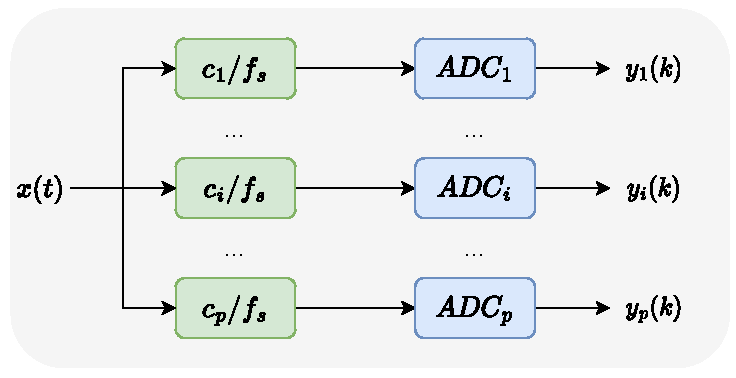
\includegraphics[width=0.8\textwidth]{Image/multi_coset.pdf}
    \caption{多陪集采样示意图}
    \label{fig:multicoset}
\end{figure}

集合 \(C = \{c_i\}_{i=1}^p\) 表示从集合 \(\{0,1,\ldots,L-1\}\) 中选择的 \(p < L\) 个不同的整数,这些整数构成了多陪集采样的模式。在多陪集采样中,选择了这些不同的整数作为时延,从而在时域上对输入信号进行了非均匀采样。这种方式的采样频率降低,有助于减少采样数据量,特别适用于宽带信号,其中信号的频谱不是均匀分布,而是集中在某些频率分量上。通过选择适当的 \(C\) 和 \(L\),可以灵活地调整采样方式,以满足信号的频谱特性和采样资源的限制。

\begin{figure}
    \centering
    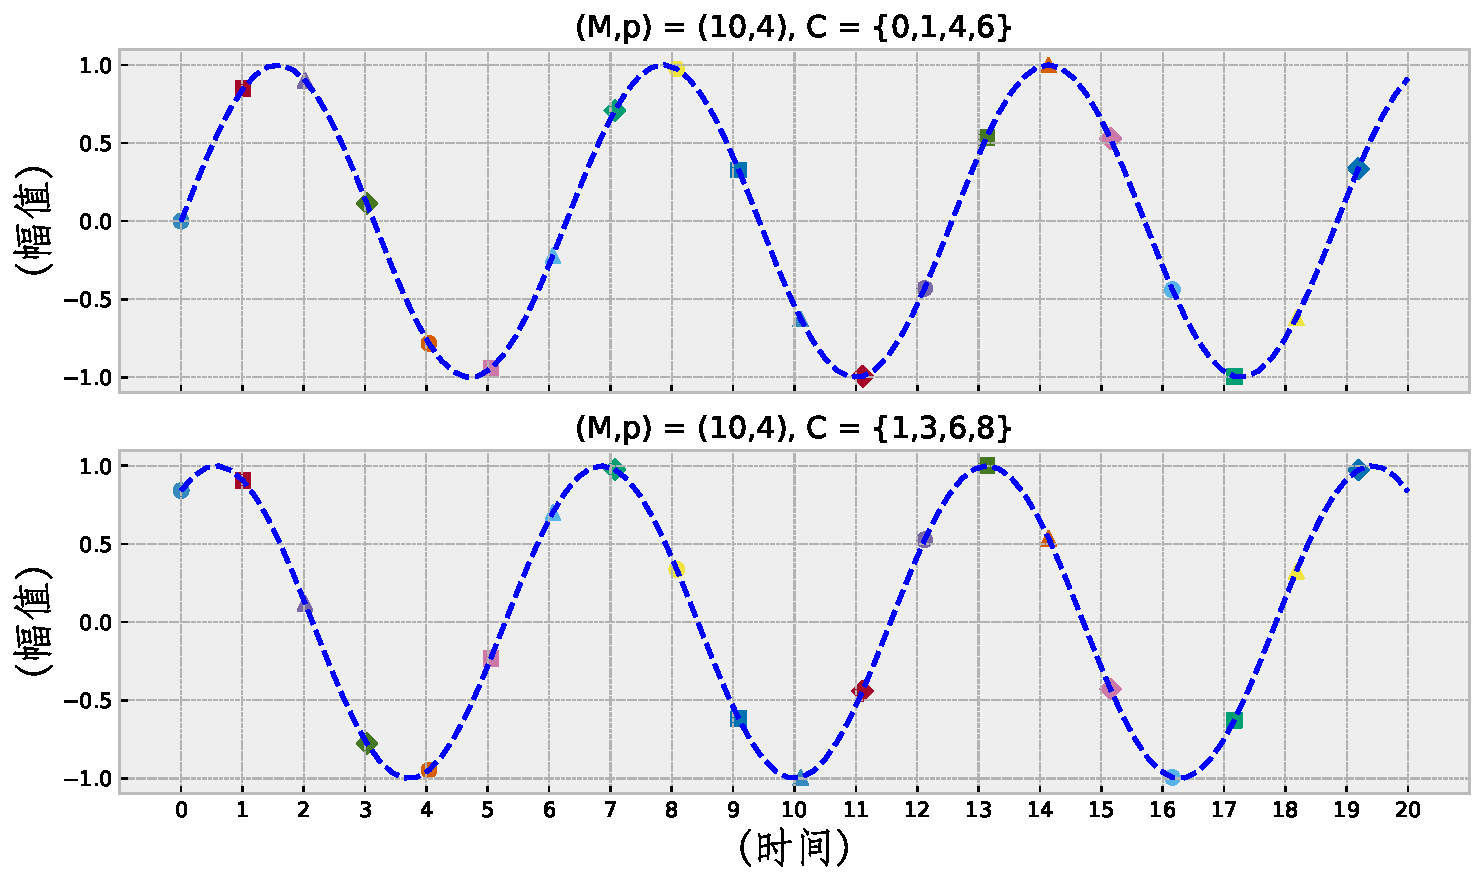
\includegraphics[width=\textwidth]{Image/mcs_process.pdf}
    \caption{多陪集采样过程示意图}
    \label{fig:multicoset_sample}
\end{figure}

图~\ref{fig:multicoset_sample}展示了多陪集采样的采样示意图,其中采样周期 \(M = 10\),采样通道数 \(p = 4\),并呈现了两种不同的采样模式,分别为 \(C = \{0,1,4,6\}\) 和 \(C = \{1,3,6,8\}\)。

在图中,圆形表示第一通道的采样点,三角形表示第二通道的采样点,正方形表示第三通道的采样点,菱形表示第四通道的采样点。通过观察图示,可以发现多陪集采样采用了一种与传统奈奎斯特采样方式不同的周期非均匀采样技术。采样模式的选择通过集合 \(C\) 中的不同整数,导致了在时域上的不同时延,形成了非均匀的采样结构。

这种多陪集采样技术的优势在于能够以较低的采样频率有效地采样宽带信号,同时通过灵活选择采样模式,适应信号频谱的稀疏性质。这样的非均匀采样方式为在资源受限的情况下实现对宽带信号的高效采样和重建提供了一种有益的途径。

\section{数据集}\label{sec:background}

% \begin{table}[htbp]
%     \centering
%     \caption{数据集概览}
%     \resizebox{\textwidth}{!}{%
%         \begin{tabular}{cm{0.4\linewidth}ccccm{0.2\linewidth}m{0.25\linewidth}}
%             \toprule
%             数据集 & 调制模式 & 样本维度 & 数据集大小 & 信噪比范围 & 特点 & 适用任务 \\
%             \midrule
%             RadioML 2016.10A & 11 类 (8PSK, BPSK,  CPFSK, GFSK, PAM4, AM-DSB, AM-SSB, 16QAM, 64QAM, QPSK, WBFM) & 2 \times 128 & 220000 & -20:2:18 & 短序列调试分类 & 传统方法与深度学习方法性能比较 \\
%             \midrule
%             RadioML 2016.10B & 10 类 (8PSK, BPSK,  CPFSK, GFSK, PAM4, AM-DSB,
%             16QAM, 64QAM, QPSK, WBFM) & 2 \times 128 & 1200000 & -20:2:18 & 短序列调制分类  (数据集更大) & 传统方法与深度学习方法性能比较 \\
%             \midrule
%             RadioML 2018.01A & 24类(OOK, 4ASK, 8ASK, BPSK, QPSK, 8PSK, 16PSK, 32PSK, 16APSK, 32APSK, 64APSK, 128APSK, 16QAM, 32QAM, 64QAM, 128QAM, 256QAM, AM-SSB-WC, AM-SSB-SC, AM-DSB-WC, AM-DSB-SC, FM, GMSK, OQPSK) & 2 \times 1024 & 2555904 & -20:2:30 & 长序列调制分类  (可模拟亚采样任务) & 可用于多种深度学习任务(调制识别、信号重构等) \\
%             \midrule
%             GBSense 2022 Basic & 13类(APSK16, APSK32, APSK64, ASK8, BPSK, OQPSK, PSK16, PSK8, QAM128, QAM16, QAM256, QAM64, QPSK) & 16 \times 1024 & 124800 & 真实环境采集信号 &欠采样宽带信号(单用户)调制分类 & 深度学习模型性能验证 \\
%             \midrule
%             GBSense 2022 Advance & 同上 & 16 \times 1024 & 102400 & 真实环境采集信号 &欠采样宽带信号(多用户)调制分类 & 多任务(包括宽带频谱感知与子带调制识别)深度学习模型性能验证 \\
%             \midrule
%             GBSense 2023 Basic & 2类(8PSK, 16QAM) & 16 \times 20 & 138240 & 真实环境采集信号 &欠采样宽带信号(单用户)调制解调 & 多任务深度学习解调(一个样本对应一个信息) \\
%             \midrule
%             GBSense 2023 Advance & 3类(QPSK, 8PSK, 16QAM) & 16 \times 20 & 500000 & 真实环境采集信号 &欠采样宽带信号(多用户)调制解调 & 多任务深度学习解调(一个样本对应多个信息)\\
%             \bottomrule
%         \end{tabular}
%     }
%     \label{tab:dataset}
% \end{table}

% 本研究使用多个开源数据集,包括由GNURadio生成的RadioML 2016.10A/B和RadioML 2018.01A,以及通过多陪集采样获取的真实宽带信号数据集GBSense 2022 Basic/Advance,以及专为解调任务设计的GBSense 2023 Basic/Advance。这些数据集为后续实验提供了可靠的基础支持。表~\ref{tab:dataset}简单介绍了这些数据集的基本信息。


% 当前,主流的AMR研究倾向于采用RadioML2016.10a数据集。该数据集数据量适中,包含一些常见的模拟和数字调制类型,如QAM、PSK、FSK和AM等。该数据集的采样点数适中,数据集大小也相对较小,适合用于验证算法的有效性。一般可用于传统算法和较为轻量的深度学习算法之间的性能比较。后续的RadioML 2016.10b数据集是对RadioML 2016.10a数据集的扩展,数据集大小更大,更适用于研究深度学习算法的鲁班性和泛化能力。而RadioML 2018.01a数据集则更为庞大,包含了24种调制类型,采样点数也增至1024,更能模拟真实环境中所采样到的信号,适用于更复杂的深度学习算法研究。

% GBSense 2022 Basic数据集通过多陪集采样获取真实宽带信号数据,包含13种调制类型,采样点数为1024,使用了8个低速的ADC进行采样,每个ADC的时延分别为16、11、1、0、27、24、37、31。各采样同一信号的同相分量和正交分量,故最终采样的信号维度为$16 \times 1024$。该数据集适用于研究亚采样宽带信号的调制识别问题。GBSense 2022 Advance数据集的采样方式与GBSense 2022 Basic相同,但采样的信号为多用户的宽带信号,即所采样的信号为多个用户的信号叠加。具体的任务是识别每个用户的调制类型及其所占的子带编号。

% GBSense 2023数据集的基本形式类似于GBSense 2022,不过其任务是对欠采样的宽带信号进行解调。相较于调制识别任务,解调任务需要识别信号的调制类型和符号长度等。在Advance版本中还需要对子带编号进行识别,因此其难度更大,同时对该任务的研究更具有实际意义。

\begin{table}[htbp]
    \centering
    \caption{数据集概览}
    \resizebox{\textwidth}{!}{%
        \begin{tabular}{m{0.3\linewidth}m{0.35\linewidth}m{0.2\linewidth}m{0.2\linewidth}m{0.15\linewidth}m{0.3\linewidth}}
            \toprule
            数据集 & 调制模式 & 样本维度 & 数据集大小 & 信噪比范围 & 适用任务 \\
            \midrule
            RadioML 2016.10A \\ (短序列) & 11 类 (8PSK, BPSK, CPFSK, GFSK, PAM4, AM-DSB, AM-SSB, 16QAM, 64QAM, QPSK, WBFM) & 2 \times 128 & 220000 & -20:2:18 & 传统方法与深度学习方法性能比较 \\
            \midrule
            RadioML 2016.10B \\ (数据集更大) & 10 类 (8PSK, BPSK, CPFSK, GFSK, PAM4, AM-DSB, 16QAM, 64QAM, QPSK, WBFM) & 2 \times 128 & 1200000 & -20:2:18 & 传统方法与深度学习方法性能比较 \\
            \midrule
            RadioML 2018.01A \\ (长序列) & 24类(OOK, 4ASK, 8ASK, BPSK, QPSK, 8PSK, 16PSK, 32PSK, 16APSK, 32APSK, 64APSK, 128APSK, 16QAM, 32QAM, 64QAM, 128QAM, 256QAM, AM-SSB-WC, AM-SSB-SC, AM-DSB-WC, AM-DSB-SC, FM, GMSK, OQPSK) & 2 \times 1024 & 2555904 & -20:2:30 & 可用于多种深度学习任务(调制识别、信号重构等) \\
            \midrule
            GBSense 2022 Basic \\ (亚采样宽带信号(单用户)调制分类) & 13类(APSK16, APSK32, APSK64, ASK8, BPSK, OQPSK, PSK16, PSK8, QAM128, QAM16, QAM256, QAM64, QPSK) & 16 \times 1024 & 124800 & 真实环境采集信号 & 深度学习模型性能验证 \\
            \midrule
            GBSense 2022 Advance \\ (亚采样宽带信号(多用户)调制分类) & 同上 & 16 \times 1024 & 102400 & 真实环境采集信号 & 多任务(包括宽带频谱感知与子带调制识别)深度学习模型性能验证 \\
            \midrule
            GBSense 2023 Basic \\ (亚采样宽带信号(单用户)调制解调) & 2类(8PSK, 16QAM) & 16 \times 20 & 138240 & 真实环境采集信号 & 多任务深度学习解调(一个样本对应一个信息) \\
            \midrule
            GBSense 2023 Advance \\ (亚采样宽带信号(多用户)调制解调) & 3类(QPSK, 8PSK, 16QAM) & 16 \times 20 & 500000 & 真实环境采集信号 & 多任务深度学习解调(一个样本对应多个信息)\\
            \bottomrule
        \end{tabular}
    }
    \label{tab:dataset}
\end{table}


本研究采用了多个开源数据集,包括基于GNURadio生成的RadioML 2016.10A/B和RadioML 2018.01A,以及通过多陪集采样技术获得的真实宽带信号数据集GBSense 2022 Basic/Advance,还有专门为解调任务设计的GBSense 2023 Basic/Advance。这些数据集为本研究的后续实验提供了坚实的基础。表~\ref{tab:dataset}概述了这些数据集的关键特点。

RadioML2016.10A数据集是当前自动调制识别(AMR)研究中的主流选择。该数据集覆盖了多种常见的模拟和数字调制类型,例如QAM、PSK、FSK和AM。数据集规模适中,采样点数合适,非常适合用于评估不同算法的有效性,尤其是在传统算法和深度学习算法的性能比较方面。RadioML 2016.10B数据集作为RadioML 2016.10A的扩展,具有更大的数据集规模,适合于研究深度学习算法的鲁棒性和泛化能力。RadioML 2018.01A数据集则更加庞大,包含了24种调制类型,采样点数增至1024,更贴近真实信号环境的复杂性,适用于更高级的深度学习算法研究。

GBSense 2022 Basic数据集通过多陪集采样技术获取了真实环境中的宽带信号数据,包含13种调制类型,采样点数为1024。该数据集采用8个低速ADC进行采样,每个ADC的时延不同,从而为研究亚采样宽带信号的调制识别问题提供了独特的数据。GBSense 2022 Advance数据集的采样方式与Basic版本相同,但它涵盖了多用户的宽带信号,为识别每个用户的调制类型及子带编号提供了数据支持。

GBSense 2023数据集延续了GBSense 2022的基本形式,但专注于宽带信号的解调任务。与调制识别任务相比,解调任务需要识别信号的调制类型和符号长度等更多信息。在其Advance版本中,还需识别子带编号,这增加了任务的难度,但也使研究更具实际意义。

综上所述,这些数据集为评估不同调制识别和解调方法提供了丰富的实验资源,是本研究得以深入探索和验证不同技术在实际场景中性能的重要基础。

\section{本章小节}\label{sec:background}
% 本章首先介绍了自动调制识别的研究背景和意义,然后分别介绍了似然比法、特征提取法和深度学习方法,最后介绍了压缩感知理论。本章的主要内容是自动调制识别的方法研究,为后续章节的内容做铺垫。
本章节综合性地介绍了数字调制信号模型、深度学习理论基础、宽带信号模型、压缩感知理论基础及调制识别相关数据集,旨在为自动调制识别领域的研究提供全面的理论和实验支持。

首先,章节深入探讨了数字调制信号模型,涵盖了幅移键控(ASK)、频移键控(FSK)、相移键控(PSK)以及正交振幅调制(QAM)。这些模型通过不同方式(振幅、频率或相位的变化)编码数字信息,为理解复杂通信系统中的信号传输提供了基础。

接着,本章节阐述了深度学习的理论基础,包括神经网络结构、激活函数、反向传播和损失函数,这些都是构建高效深度学习模型的关键要素。深度学习在自动调制识别中展现出的强大能力,使其成为处理复杂信号识别任务的有效工具。

此外,章节详细介绍了宽带信号模型,揭示了宽带信号作为多个子带信号叠加的特性。这一模型对于处理和分析现代通信系统中的高频宽带信号至关重要。

本章还系统地介绍了压缩感知理论,这是一种处理大规模数据的有效技术。首先,简要介绍了压缩感知理论的基本概念,随后深入探讨了信号的稀疏表示,这是压缩感知的核心概念之一。稀疏表示强调了信号可以在某些基下高效表示的特点,为降低采样需求提供了理论基础。最后,详细解释了多陪集采样的基本原理,这是一种实现高效信号采样的方法,尤其适用于处理高维度和大规模数据集,如宽带信号。

最后,本章概述了几个关键数据集,包括RadioML 2016.10A/B、RadioML 2018.01A以及GBSense 2022/2023。这些数据集为自动调制识别的研究提供了实验基础,覆盖了基本的调制类型识别到复杂的宽带信号处理任务。

综合这些理论和实践资源,本章为自动调制识别领域的研究奠定了坚实的理论基础和实验准备,为未来在这一领域的深入研究和探索提供了必要的背景和知识支持。